\documentclass[12pt]{article}

\usepackage{amssymb,amsmath,amsthm}
\usepackage{graphicx} % Package for including figures
%\usepackage{psfrag,color}

\theoremstyle{definition}
\newtheorem{thm}{Theorem}[section]
\newtheorem{lem}[thm]{Lema}
\newtheorem{prop}[thm]{Proposition}
\newtheorem*{cor}{Corrolary}

\theoremstyle{definition}
\newtheorem{defn}{Definition}[section]
\newtheorem{conj}{Conjecture}[section]
\newtheorem{exmp}{Example}[section]


\title{Report: Homework 5 Math/CS 471}
\author{Teo 'The Real' Brandt and Brennan 'Buckshot' Collins}
\date{\today}   % Activate to display a given date or no date


\begin{document}
\maketitle

\begin{abstract}
This report will explore the process used to simulate the interaction of objects (hereafter referred to as angry-birds) in a two-dimensional spacial coordinate system. The dynamics of these angry birds will be described by ordinary differential equations and the successive location of each bird will be updated using the forth-oder Runge-Kutta method.
\end{abstract}

\begin{figure}[h]

\includegraphics[width=8cm]{angrybirds}
\end{figure}

\section{Runge-Kutta}

\cite{HW}Runge-Kutta 4 is a numerical technique used to approximate the solution to first order ordinary differential equations of the form
\[
\frac{dy}{dt}=f(x,y)\text{,  }y(0)=y_{0}
\]
The approximation to this function can be first visualized as the first five terms of the Taylor expansion
\[
\frac{dy}{dx}=f(x,y)\text{ and }x_{i+1}-x_{i}=h
\]
\[
y_{i+1}=y_{i}+f(x_{i},y_{i})h+\frac{1}{2!}f'(x_{i},y_{i})h^{2}+\frac{1}{3!}f''(x_{i},y_{i})h^{3}+\frac{1}{4!}f'''(x_{i},y_{i})h^{4}
\]
The Runge-Kutta 4 method is based on this expression and has the form
\[
y_{i+1}=y_{i}+\frac{1}{6}(k_{1}+2k_{2}+2k_{3}+k_{4})h
\]
Where
\[k_{1}=f(x_{i},y_{i})\]
\[k_{2}=f(x_{i}+\frac{1}{2}h\text{, }y_{i}+\frac{1}{2}k_{1}h)\]
\[k_{2}=f(x_{i}+\frac{1}{2}h\text{, }y_{i}+\frac{1}{2}k_{2}h)\]
\[k_{2}=f(x_{i}+\frac{1}{2}h\text{, }y_{i}+k_{3}h)\]
In this report the first variable of \(f\), \(x\), is describing the time while the second variable \(y\) describes the spacial orientation. The solution \(y_{i+1}\) is the location at the next time step. More specific dynamics will be discussed in the next section of this report.
\section{Angry Birds: Problem Formulation}
Consider the existence of a bird feeder who's name is James. James has a pre-determined, time-dependent path described by the circle
\[
C(t)=(\sin(2t),\cos(2t))
\]
Also, we have a leader bird. This bird's trajectory depends only on the location of James. The leader will try to minimize the distance to James at each subsequent time step with some attraction \(\gamma_{1}\)
\[
\frac{dB_{1}}{dt}=\gamma_{1}(C(t)-B_{1}(t))
\]
The other birds in the flock \(B_{k}\), \(k=2,...,n_{Birds}\) are dependent on the distance they are from the leader as well as on the attraction they have to the leader
\[
\frac{dB_{k}}{dt}=\gamma_{2}(B_{1}(t)-B_{k}(t))\text{,  }k=2,...,n_{Birds}
\]
There are two other mechanisms that affect the rate of the follower birds with one being the tendency of birds of a feather to flock together and maneuverability. The birds will be attracted to their center of gravity, \(\={B}\) at some rate \(\kappa\)
\[
\kappa(\={B}(t)-B_{k}(t))\text{,  }k=2,...,n_{Birds}
\]
Also, in order for the birds to be able to move around freely there is some repulsion that is exhibited by the closest neighbors by
\[
\sum_{l=1}^{L}\rho\frac{(B_{k}(t)-B_{l}(t))}{(B_{k}(t)-B_{l}(t))^{2}+\delta}\text{,  }k=2,...,n_{Birds}
\]


\section{Procedure}
In order to make sense out of the dynamics described in the previous section two cases are provided. The first case is that when the bird feeder's path is described by a circle of radius 2 (\(C(t)=(\sin(2t),\cos(2t))\)). The second case is when the bird feeder is stationary, and located at the origin.

The parameters used in the simulations are:
\[N=10\text{ Ten birds total, including the leader}\]
\[\gamma_{1}=20\text{ A moderately hungry bird-leader}\]
\[\gamma_{2}=30\text{ A very charismatic bird-leader}\]
\[\kappa=1\text{ A spread out flock (for ease of viewing)}\]
\[\rho=1\text{ A friendly flock that has the ability to move closely}\]
\[\delta=0.001\text{ Again, a friendly flock}\]
\newpage
\begin{figure}[h]
\caption{Circular path of the feeder}
\centering
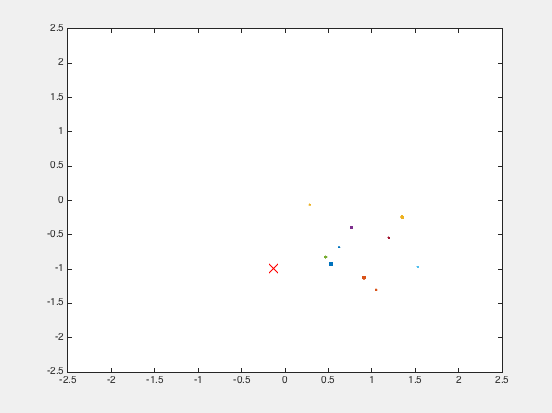
\includegraphics[width=0.5\textwidth]{trial1}
\end{figure}
\begin{figure}[h]
\caption{Stationary path of the feeder}
\centering
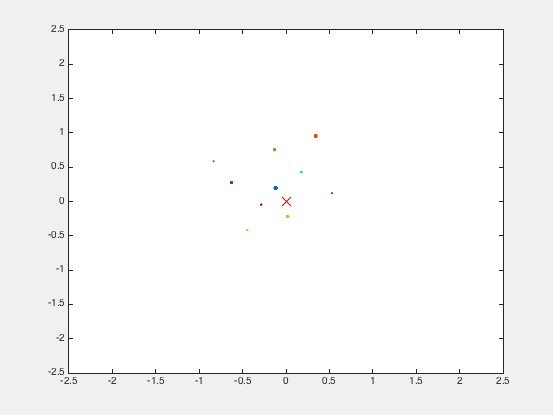
\includegraphics[width=0.5\textwidth]{trial2}
\end{figure}
\\
\newpage
\section{Appendix}
\indent In order to compile and execute the code for this assignment first enter the directory:
\\
\begin{center}
\textit{~/Homework/Homework5/Code/}
\end{center}
\\
and then use the following command:
\\
\begin{center}
\textit{\$ run.sh}
\end{center}
\\
following this command two successive videos will play, demonstrating the simulations described above

\newpage
\begin{thebibliography}{9}
\bibitem{HW} 
Daniel Appelo
\textit{Homework 3}. 
referenced Oct. 15, 2015

\end{thebibliography}

\end{document} 